%%%%%%%%%%%%%%%%%%%%%%%%%%%%%%%%%%%%%%%%%%%%%%%%%%%%%%%%%%%%%%%%%%%%%%%%%%
%
%    GemPhase1.tex  
%
%    GEMINI OBSERVATORY
%    PHASE I OBSERVING PROPOSAL TEMPLATE 
%    FOR SEMESTER 2015A
%
%    Version 1.5, August 30, 2013
%
%    Guidelines and assistance
%    =========================
%     2015A Announcement Web Page:
%
%         http://www.gemini.edu/sciops/observing-gemini/2015a-call-proposals
%
%    Please contact the Gemini Help Desk if you need assistance. 
%    http://www.gemini.edu/sciops/helpdesk/submit-general-helpdesk-request
%
%%%%%%%%%%%%%%%%%%%%%%%%%%%%%%%%%%%%%%%%%%%%%%%%%%%%%%%%%%%%%%%%%%%%%%%%%%%


% Please do not modify or delete this line.
\documentclass[11pt]{article}
\usepackage{GemPhase1_15A}
\usepackage{subfigure}
\usepackage{natbib}

% Please do not modify or delete this line.
\begin{document}

%%%%%%%%%%%%%%%%%%%%%%%%%%%%%%%%%%%%%%%%%%%%%%%%%%%%%%%%%%%%%%%%%%%%%%

% In the following "essay question" sections, the delimiting pieces of
% markup (\justification, \expdesign, etc.) act as LaTeX \section*{}
% commands.  If the author wanted to have numbered subsections within
% any of these, LaTeX's \subsection could be used.
%
% DO NOT REDUCE THE FONT SIZE, and do not otherwise fiddle with the
% format to get more on a page.  We will reset any changes back to the
% default font.

%%%%%%%%%%%%%%%%%%%%%%%%%%%%%%%%%%%%%%%%%%%%%%%%%%%%%%%%%%%%%%%%%%%%%

% SCIENTIFIC JUSTIFICATION
%
% Give the scientific justification for the proposed observations, including
% the overall significance to astronomy.  As requested by the reviewers, 
% THE SCIENTIFIC JUSTIFICATION IS LIMITED TO ONE PAGE 
% EXCLUDING REFERENCES, with up to two additional pages
% for references, tables, figures (no more than three), and captions. 
% This section should be a high-level description of the observations and
% the  fundamental problem that they will address.  The Experimental Design
% section can be used to describe the overall observational program, including 
% sample selection, data analysis, etc. The Technical Case can include details 
% about the instruments, conditions, and exposure times required.
%
% If you wish to use our "reference" environment, follow the following
% example (journal commands are compatible with AASTeX v4.0):
%
%\begin{references}
%\reference Armandroff \& Massey 1991 \aj, 102, 927.
%\reference Berkhuijsen \& Humphreys 1989 \aap, 214, 68.
%\reference Massey 1993 in Massive Stars: Their Lives in the 
% Interstellar Medium (Review), ed. J. P. Cassinelli and E. B. 
% Churchwell, p. 168.
%\reference Massey \& Armandroff 1999, in prep.
%\end{references}

% In order to include an EPS plot  you can use the LaTeX "figure" environment.
% The plot file is included with the \plotone{FILENAME} command; two
% side-by-side plot files can be included by typing
% \plottwo{FILENAME1}{FILENAME2}.  Use \caption{} to specify a caption.
% The \epsscale{} command can be used to scale \plotone plots if they
% appear too large on the printed page.  
%
% \begin{figure}
% \epsscale{0.85}
% \plotone{sample.eps}
% \caption{Sample figure showing important results.}
% \end{figure}
%
% If you need to rotate or make other transformations to a figure, you
% may use the \plotfiddle command:
% \plotfiddle{PSFILE}{VSIZE}{ROTANG}{HSCALE}{VSCALE}{HTRANS}{VTRANS}
% \plotfiddle{sample.eps}{2.6in}{-90.}{32.}{32.}{-250}{225}
% where HSCALE and VSCALE are percentages and HTRANS and VTRANS are
% in PostScript units, 72 PS units = 1 inch.
%
%
% Or use includegraphics for example
% \includegraphics[angle=0,scale=.6]{fig1.png}
%

\sciencejustification    % Do not delete this command.
Type Ia supernovae (SNe Ia) are thermonuclear explosions of a white dwarf in a binary system. They have been proven to be excellent distance indicators for constraining cosmological parameters, and are major contributors to the cosmic chemical enrichment. There remain, however, several open questions regarding the physics of the explosions that still need to be addressed, e.g. the mass at the time of white dwarf, the nature of the progenitor binary system, and the explosion physics. We propose to obtain a time-series of near-infrared (NIR) spectra of the closest SN Ia in four decades - 2014J - from 400 -- 500\,days past explosion. This will allow us to study the core of the exploded object, which in turn can be used to shed light on the progenitor white dwarf. 

\textbf{The power of nebular spectroscopy} Most data on SNe Ia is collected during the photospheric phase. In contrast, the late time, nebular phase ($\gtrsim$ 100 days after maximum) has been observed much less frequently as most objects are too faint. At these epochs the ejecta is optically thin at most wavelengths and no continuum is produced. Instead, the spectrum is dominated by forbidden line transitions of iron-group elements. The strength and shape of the lines provides information about the abundance stratification and density distribution in the core of the exploded object. High-quality optical spectra at up to 400 days past maximum have been used to infer the 3-D abundance distribution in the ejecta (Maeda et al. [2010]).

\textbf{Exploring the late time plasma state of SNe Ia} Recent optical observations of the also very nearby SN2011fe (Taubenberger et al. [2015]) demonstrate a puzzling behaviour of this SN at very late epochs ($>$+1000d). The previously prominent [Fe III] feature at 4700 \AA\ has completely faded. Instead, most of the emission is probably in [Fe II] lines. This suggests a significant change in the ionisation state. At the same time, the emission arises from relatively high-excitation lines, showing that the general evolution of the late-time plasma state in SNe Ia is very poorly understood. This becomes even more interesting if one compares the observed behaviour to theoretical predictions. At late epochs the ejecta begins to cool as the radioactive heating decreases whereas the cooling curve flattens. Once the ejecta temperature decreases below a critical threshold ($< 1500$\,K), the optical and NIR flux is expected to drop dramatically, which is known as the Infrared Catastrophe (IRC; Axelrod [1980]). Although theoretical models predict this IRC to happen around 500 \,d, it has never been observed in any of the few SNe that have been followed up photometrically to sufficiently late phases (Leloudas et al. [2009], Kerzendorf et al. [2014]; for an example see Figure~\ref{fig:11fe}). NIR spectra in the range of +400 - +500 days will provide valuable information on the ionisation and excitation state of the ejecta as well as the temperature in the core. This will allow us to judge how close SN2014J is to undergoing an IRC. One possible reason for the absence of an IRC might be clumping of ejecta which keeps the local temperature above the threshold. Line morphologies in high-S/N NIR spectra can provide evidence for clumping in the ejecta.  Particularly suited for this endeavour is the unblended [Fe II] feature at 1.644\,$\mu$m (see Figure \ref{fig:Mspec}).  




\textbf{Shifting lines in late time spectra}
Another puzzling feature seen in very late-time ($>1000$\,days) spectra of SN 2011fe is a global shift of iron-group element features by 4000\,km\,s$^{-1}$ when compared to spectra at 300\,days (Taubenberger et al. [2015]; see Figure \ref{fig:11fe}). Normally, line shifts in nebular spectra are explained by asymmetries in the ejecta of the SN, which can provide powerful constraints on the progenitor system and explosion mechanism. However, in the case of SN2011fe the geometric interpretation is not straightforward, as neither the size of the  shift nor its temporal evolution between 300 and 1000\,days can be explained in this way. Hence, the origin of the phenomenon currently remains unknown. There are no published spectra of SN2011fe between +331 and +1034\,d, hence one cannot constrain what the driving mechanism for this line shift is. Spectra of a normal SN~Ia like SN2014J at regular intervals and at intermediate epochs can shed light onto whether this is a sudden or a gradual change. 

\newpage

\begin{figure}
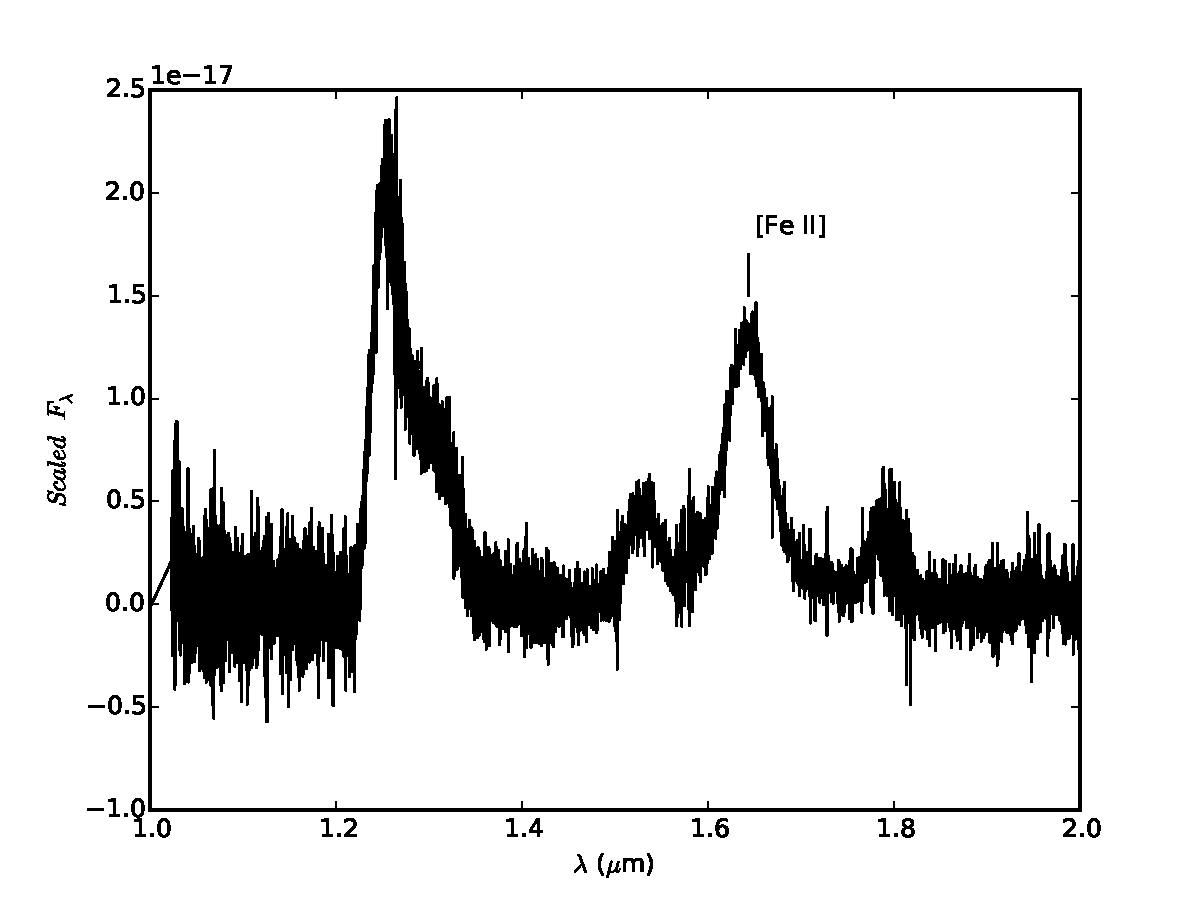
\includegraphics[width=.7\textwidth]{../13aa.pdf}
%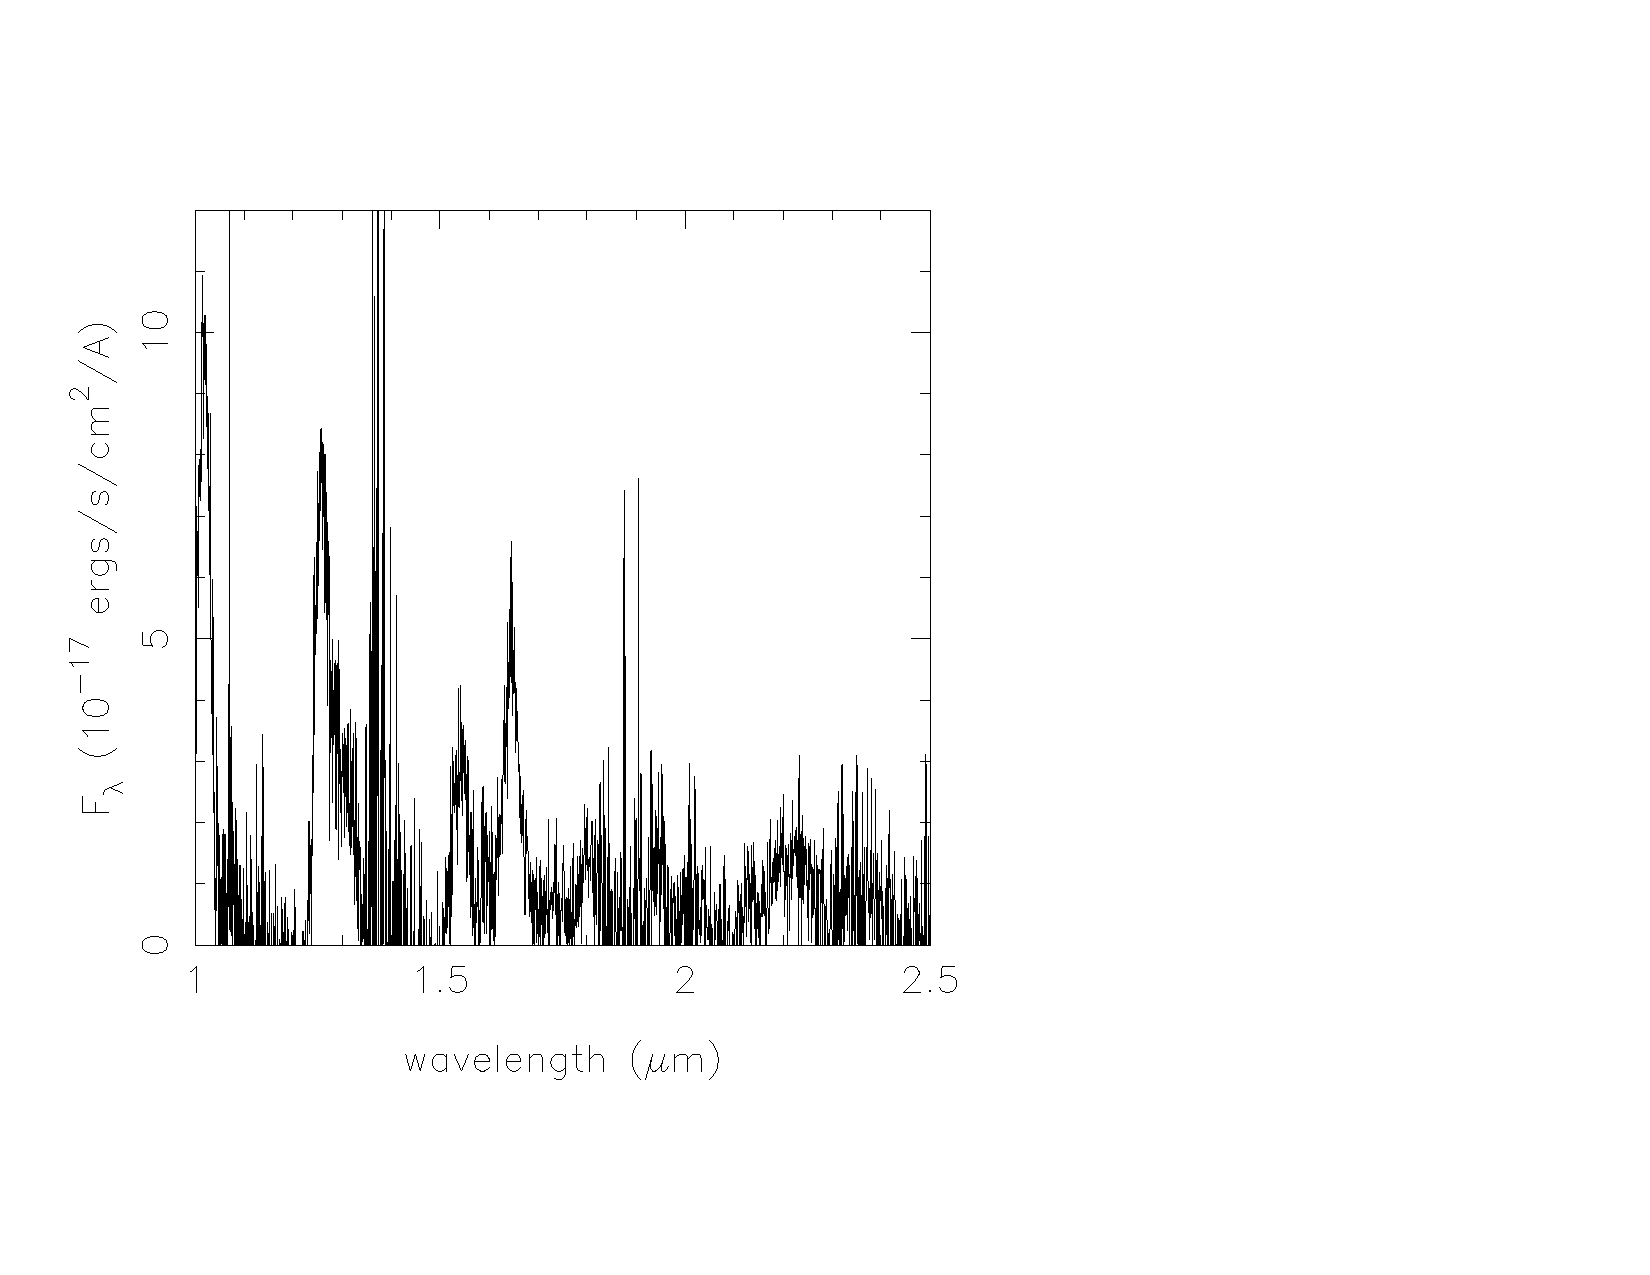
\includegraphics[width=240mm, height = 70mm]{../0570fig1.pdf}
\caption{A nebular phase spectrum of SN2013aa (Maguire et al. in prep). The [Fe II] feature at 1.644 $\mu$m is marked. }%The figure shows the spectral energy distribution from the B to the K band for SN2014J (Johannsson et al. [2014]). The spectra are at phases of , +5d,+31d, +126d}
\label{fig:Mspec}
\end{figure}

\begin{figure}
\centering
\begin{subfigure}{\textwidth}
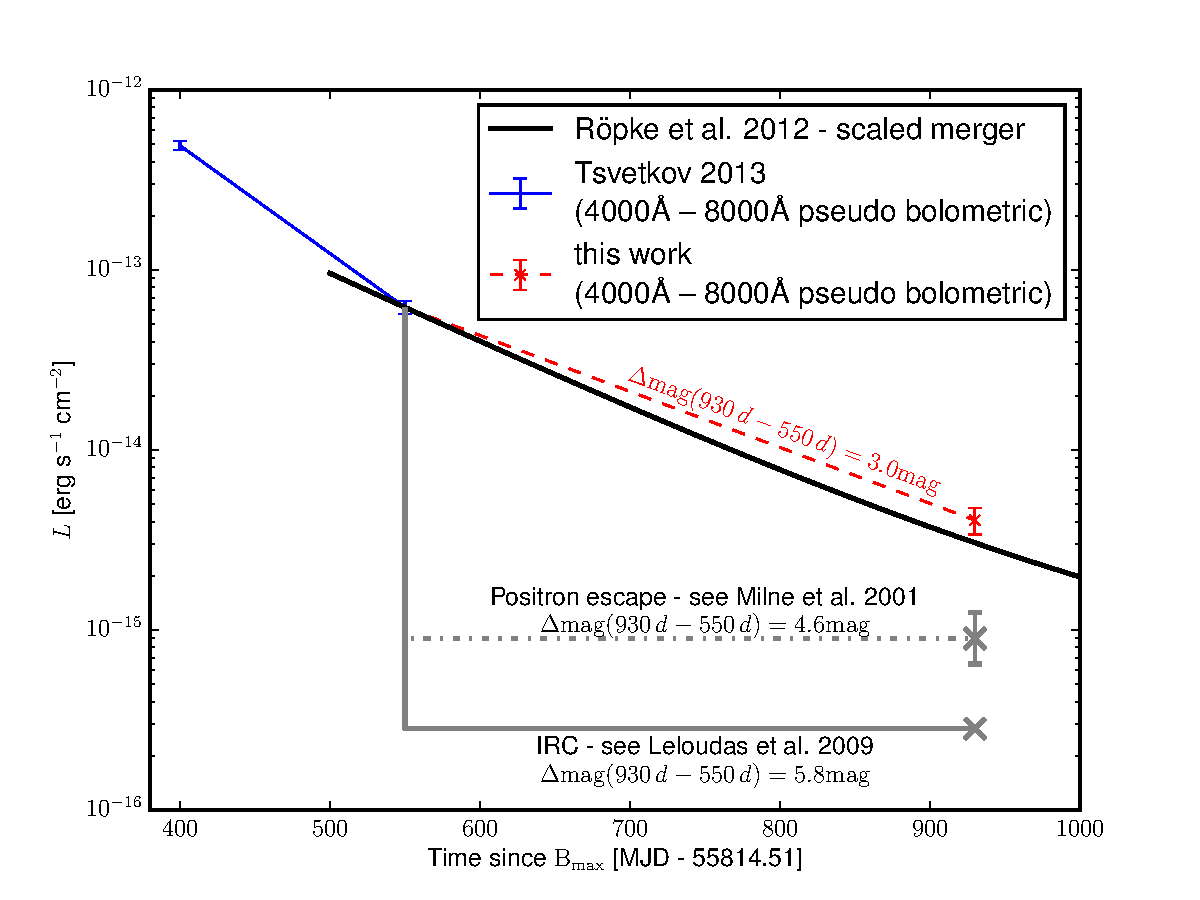
\includegraphics[width=.48\textwidth, trim= 0 0 35 0]{../sn11fe_bolom.pdf}
\end{subfigure}
~
\begin{subfigure}{\textwidth}
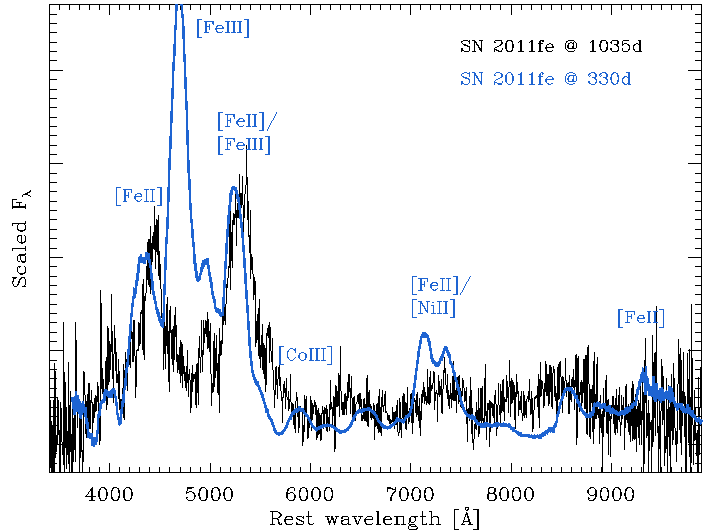
\includegraphics[width=.48\textwidth, trim= 0 0 10 0]{../11fe_II.pdf}
\label{sfig:2b}
\end{subfigure}
\caption{\emph{Left}: The late time bolometric light curve of SN2011fe (Kerzendorf et al. [2014]). There is no evidence for an IRC \emph{Right}: A comparison of the SN2011fe spectra at +331 and +1034\,d showing the line shift at the later epoch. }
\label{fig:11fe}
\end{figure}

\newpage

\begin{thebibliography}{99}
\bibitem[\protect\citeauthoryear{Ashall et al.}{2014}]{2014MNRAS.445.4427A} 
Ashall C., Mazzali P., Bersier D., Hachinger S., Phillips M., Percival S., 
James P., Maguire K., 2014, MNRAS, 445, 4427

\bibitem[\protect\citeauthoryear{Axelrod}{1980}]{Axelrod80} 
Axelrod T.~S., 1980, PhDT 

\bibitem[\protect\citeauthoryear{Blondin et 
al.}{2012}]{Blondin2012} Blondin S., et al., 2012, AJ, 143, 126 

\bibitem[\protect\citeauthoryear{Chomiuk et 
al.}{2012}]{2012ApJ...750..164C} Chomiuk L., et al., 2012, ApJ, 750, 164 

\bibitem[\protect\citeauthoryear{Diamond, Hoeflich, 
\& Gerardy}{2014}]{Diamond2014} Diamond T., Hoeflich P., Gerardy C.~L., 2014, arXiv, arXiv:1410.6759 

\bibitem[\protect\citeauthoryear{Foley et al.}{2014}]{2014MNRAS.443.2887F} 
Foley R.~J., et al., 2014, MNRAS, 443, 2887

\bibitem[\protect\citeauthoryear{Leloudas et 
al.}{2009}]{2009A&A...505..265L} Leloudas G., et al., 2009, A\&A, 505, 265 

%\bibitem[\protect\citeauthoryear{Maeda et al.}{2011}]{Maeda2011} 
%Maeda K., et al., 2011, MNRAS, 413, 3075 



\bibitem[\protect\citeauthoryear{Li et al.}{2011}]{2011Natur.480..348L} Li 
W., et al., 2011, Natur, 480, 348 
\bibitem[\protect\citeauthoryear{Maeda et al.}{2010}]{Maeda2010} 
Maeda K., et al., 2010, Natur, 466, 82 

\bibitem[\protect\citeauthoryear{Marion et al.}{2015}]{2015ApJ...798...39M} 
Marion G.~H., et al., 2015, ApJ, 798, 39 

\bibitem[\protect\citeauthoryear{Mazzali et 
al.}{1998}]{Mazzali1998} Mazzali P.~A., Cappellaro E., Danziger 
I.~J., Turatto M., Benetti S., 1998, ApJ, 499, L49 

\bibitem[\protect\citeauthoryear{Mazzali et 
al.}{2014}]{2014MNRAS.439.1959M} Mazzali P.~A., et al., 2014, MNRAS, 439, 
1959 




 \bibitem[\protect\citeauthoryear{Patat et al.}{2014}]{2014arXiv1407.0136P} 
Patat F., et al., 2014, arXiv, arXiv:1407.0136



\bibitem[\protect\citeauthoryear{Shappee et 
al.}{2013}]{Shappee2013} Shappee B.~J., Stanek K.~Z., Pogge R.~W., 
Garnavich P.~M., 2013, ApJ, 762, LL5 

\bibitem[\protect\citeauthoryear{Taubenberger et 
al.}{2015}]{T15} Taubenberger S., et al., 2015, MNRAS, 448, 
L48 


\end{thebibliography}

%%%%%%%%%%%%%%%%%%%%%%%%%%%%%%%%%%%%%%%%%%%%%%%%%%%%%%%%%%%%%%%%%%%%%

% EXPERIMENTAL DESIGN
%
% THE EXPERIMENTAL DESIGN IS LIMITED TO ONE PAGE WITH 
% NO ADDITIONAL FIGURES.  Describe your overall observational program.  
% How will these observations contribute toward the accomplishment of the goals 
% outlined in the science justification?  Include information such as why the specific 
% targets were selected, the sample size, the analysis, etc.  Describe any necessary
% calibrations in addition to the baseline calibrations.

\expdesign    % Do not delete this command.
SN2011fe was another extremely close SN Ia (twice the distance as SN 2014J). This event  has provided and is providing unique insights into SN Ia physics (e.g. Li et al. 2011, Chomiuk et al. 2012 Shappee et al. 2013 Mazzali et al. 2014 , Kerzendorf et al. 2014, Taubenberger et al. 2015), but also shows which observations are missing to complete some of the puzzles. Thus the closest SN Ia in more than four decades - SN 2014J - gives us the opportunity to make good for some of the missed observations. As some of these results were not available at the time of the last regular proposal deadline, we believe that the very modest request of time that we need to obtain a complete dataset for SN2014J justifies the FT mode application. Here, we propose a spectroscopic follow-up of SN2014J with regular cadence in the nebular phase in the near infrared (NIR; $0.8 - 2.2 \mu$m) between +400 to +500 days with GNIRS. 

This proposal is embedded in an observing campaign to get a comprehensive optical-NIR data set in order to study the late time properties of SN2014J. In addition to this experiment, we also propose photometric observations in the optical and NIR on the Himalayan Chandra Telescope (HCT). This will allow us to get a late time (pseudo)-bolometric light curve which can elucidate the configuration of the magnetic field in the ejecta. In addition, we will complete the dataset with optical spectroscopy obtained with the GTC Osiris instrument. Finally, an excellent dataset for the early time observations of SN2014J exists with a spectral time series in the UV, optical and NIR including multi-band photometry and polarimetry available publicly (Ashall et al. [2014], Foley et al. [2014], Marion et al. [2014], Patat et al. [2014]).
		 	 	 		
			
				
					
The proposed NIR GNIRS spectrum will allow us to verify the concepts outlined in the science justification. In particular, we intend to address the following questions: 

\begin{itemize}
\item Measure emission line strengths and ratios to determine the ionisation and excitation state of the ejecta and the temperature of the electron gas.
\item Measure line positions and profiles to infer the geometry of the emitting region (particularly using the unblended [Fe II] 1.644\,$\mu$m line).
\item Probe if there is any evolution in these quantities between 400 and 500 days.
\end{itemize}

The nebular spectra of SNe Ia are dominated by doppler-broadened ($\approx 5000$\,km\,s$^{-1}$) forbidden emission lines. Thus we propose for a low-resolution (R=700-800) cross-dispersed spectra. For each individual spectrum, we aim to model the shapes of lines with a relatively high accuracy and thus require a S/N of $\approx 50$ in the line peaks. 

While many known processes in the nebular phase change over relatively long time scales (on the order of several 100\,days), the infrared catastrophe (as one of our key science drivers) is believed to happen over a few weeks. To capture any change in the plasma state, we believe that a cadence of  $\sim$ 30 - 50 days is a good compromise. Hence, we propose to obtain 3 NIR spectra between the months of March and May. 

\newpage

%%%%%%%%%%%%%%%%%%%%%%%%%%%%%%%%%%%%%%%%%%%%%%%%%%%%%%%%%%%%%%%%%%%%%

% TECHNICAL CASE
%
% THE TECHNICAL CASE IS LIMITED TO ONE PAGE WITH NO
% ADDITIONAL FIGURES.  Also justify the instrument configuration, the exposure times 
% and the constraints requested (seeing, cloud cover, sky brightness and 
% if appropriate water vapor and elevation).  
% Specify the total time needed (including overheads), and the minimum requested 
% time. If you are applying for instruments on both Gemini North and Gemini South,
% please state the time request for each site.

\technicaldescription    % Do not delete this command.
We would like 10 exposures of 120 seconds  each per night. A total on source exposure time of 20 mins  gives us an S/N of $\sim$ 30 in the line at $\sim 1.54 \mu$m (see ITC pdf attached ). 
We would require the same number of exposures for the same duration off source. Hence the total time on and off source is 40 mins. 

For each such set of  exposures, the acquisition time is 12 mins. The readout time for each exposure is 9 seconds. Hence for 10 X 2 exposures the total readout time is 180s. 
Hence, in total we request for 1 hour for each night (using a conservative estimate for overheads), and a total of 3 hours for the period of March to May. 

We would like to use the cross-dispersed mode in order to obtain a complete spectrum from 0.8 to 2.5 $\mu$m. Recently published observations of SN2005df (Diamond et al. [2014]) using GNIRS have also used cross-dispersion mode to get a complete spectrum from 0.8-2.4 $\mu$m.

The observations can be carried out during any phase of the moon. Details of the ITC are attached. 

Based on the fast turnaround schedule we would prefer observations in April on the 14th and in May on either 25th or 26th and on any of the nights scheduled in March. However, any other nights as well would be suitable. 
\bigskip

%%%%%%%%%%%%%%%%%%%%%%%%%%%%%%%%%%%%%%%%%%%%%%%%%%%%%%%%%%%%%%%%%%%%%

% BAND 3 INFORMATION
% There is a limit of half a page of printed text.
% If you are applying for queue time, your ranking may place the program in 
% Band 3.  Band 3 observations are used to fill the queue when no Band 1 or 2 
% programs are available.  Successful Band 3 programs generally use poorer than 
% median observing conditions, have targets away from the most popular 
% regions of the sky, do not require strict timing or other constraints, 
% and do not require special instrument configurations.  Describe the changes
% you will make to the program to allow it to be successful in Band 3 in
% the \bandthreeplan section, or write "This program is not suitable for band 3"  
% or "This is not a queue request".  If a Band 3 allocation is acceptable and 
% the total Band 3 time request is different from the standard request, then 
% give the Band 3 time request for each partner and update the time requested
%  from each site.

\bandthreeplan    % Do not delete this command.

This program is not suitable for band 3.

\bigskip

%%%%%%%%%%%%%%%%%%%%%%%%%%%%%%%%%%%%%%%%%%%%%%%%%%%%%%%%%%%%%%%%%%%%%

% CLASSICAL PROGRAM INFORMATION
% There is a limit of half a page of printed text.
% If you are applying for classical time on Gemini, please 
% define a backup program in case the weather is worse than
% the observing conditions in the proposal.  Enter your classical backup 
% in the \classicalbackup section, or write "The program as specified is 
% suitable for poor conditions, or "This is not a classical request".

\classicalbackup    % Do not delete this command.
 
This is not a classical request

\bigskip

%%%%%%%%%%%%%%%%%%%%%%%%%%%%%%%%%%%%%%%%%%%%%%%%%%%%%%%%%%%%%%%%%%%%%

% DUPLICATE OBSERVATIONS
% A search of the Gemini Science Archive 
% (http://www1.cadc-ccda.hia-iha.nrc-cnrc.gc.ca/gsa/) will reveal whether
% Gemini has previously been used to observe your targets using similar or
% identical observing setups.  If there are duplicate observations, please
% justify why new observations should be taken in the \justifyduplications
% section.  If the Archive search finds no duplicates, please enter
% ``The GSA search revealed no duplicate observations''.

\justifyduplications

The GSA contains observations of SN 2014J. However, as this is a transient event the existing can not be used to fulfill our science goals

\bigskip

%%%%%%%%%%%%%%%%%%%%%%%%%%%%%%%%%%%%%%%%%%%%%%%%%%%%%%%%%%%%%%%%%%%%

%  PUBLICATIONS
% 
% Enter a list of publications written by the PI and Co-Is that support 
% the current application. Use standard tex such as for the References section.

\publications          % Do not delete this command.
\begin{thebibliography}{99}
\bibitem[\protect\citeauthoryear{Taubenberger et 
al.}{2015}]{T15} Taubenberger S., et al., 2015, MNRAS, 448, 
L48 

\bibitem[\protect\citeauthoryear{Kerzendorf et 
al.}{2014}]{K14} Kerzendorf W.~E., Taubenberger S., 
Seitenzahl I.~R., Ruiter A.~J., 2014, ApJ, 796, LL26

\bibitem[\protect\citeauthoryear{Maguire et 
al.}{2014}]{KM14} Maguire K., et al., 2014, MNRAS, 444, 3258
\end{thebibliography}
\bigskip

%%%%%%%%%%%%%%%%%%%%%%%%%%%%%%%%%%%%%%%%%%%%%%%%%%%%%%%%%%%%%%%%%%%%


% OTHER FACILITIES AND PAST GEMINI USE
%

% List any applications to non-Gemini facilities that are related to this proposal.
% For each of these other facilities, indicate the nature
% of the observations (yours or those of others), and describe the
% importance of the observations proposed here in the context of the
% entire program. Or write: "There are no non-Gemini related proposals".

\otherfacilities    % Do not delete this command.

\begin{itemize}
\item Himalayan Chandra Telescope (HCT) - multi-epoch optical and NIR photometry of SN 2014J
\item Gran Telescopio CANARIAS (GTC) - multi-epoch optical spectroscopy SN 2014J
\end{itemize}

\bigskip

% List in the Table below allocations of Gemini telescope time  to the 
% Principal Investigator during the past 2 years (e.g. GN-2011A-Q-999), 
% the amount of time awarded (e.g. 12 hrs), 
% the percentage of this that was useful (e.g. 80), 
% and text describing the current state of any data obtained (e.g. Data reduced).  

\thepast    % Do not delete this command.

The PI does not have any previous Gemini time
%\begin{table}[h]
%\begin{center}
%\begin{tabular}{llcl}
%Reference & Allocation & \% Useful & Status of previous data \\
%\hline
% &  &  & \\
%\hline
%\end{tabular}
%\end{center}
%\end{table}

\bigskip

%%%%%%%%%%%%%%%%%%%%%%%%%%%%%%%%%%%%%%%%%%%%%%%%%%%%%%%%%%%%%%%%%%%%%%%%%%%


% ITC Attachments
%

% Use the Gemini Integration Time Calculator (ITC) for a typical source for each 
% instrument requested, see
% http://www.gemini.edu/sciops/instruments/integration-time-calculators
% Save the ITC output as a PDF file and include that in this section. The ITC pages 
% will not count against the page limits.  You may either merge the ITC PDF output 
% to the PDF version of this document or include the ITC PDF output
% using \includepdf, eg.
%
% \includepdf[pages={-}]{ITCoutput.pdf}
%
% See the PIT FAQ (http://www.gemini.edu/node/11087/) for additional suggestions.

\itcresults

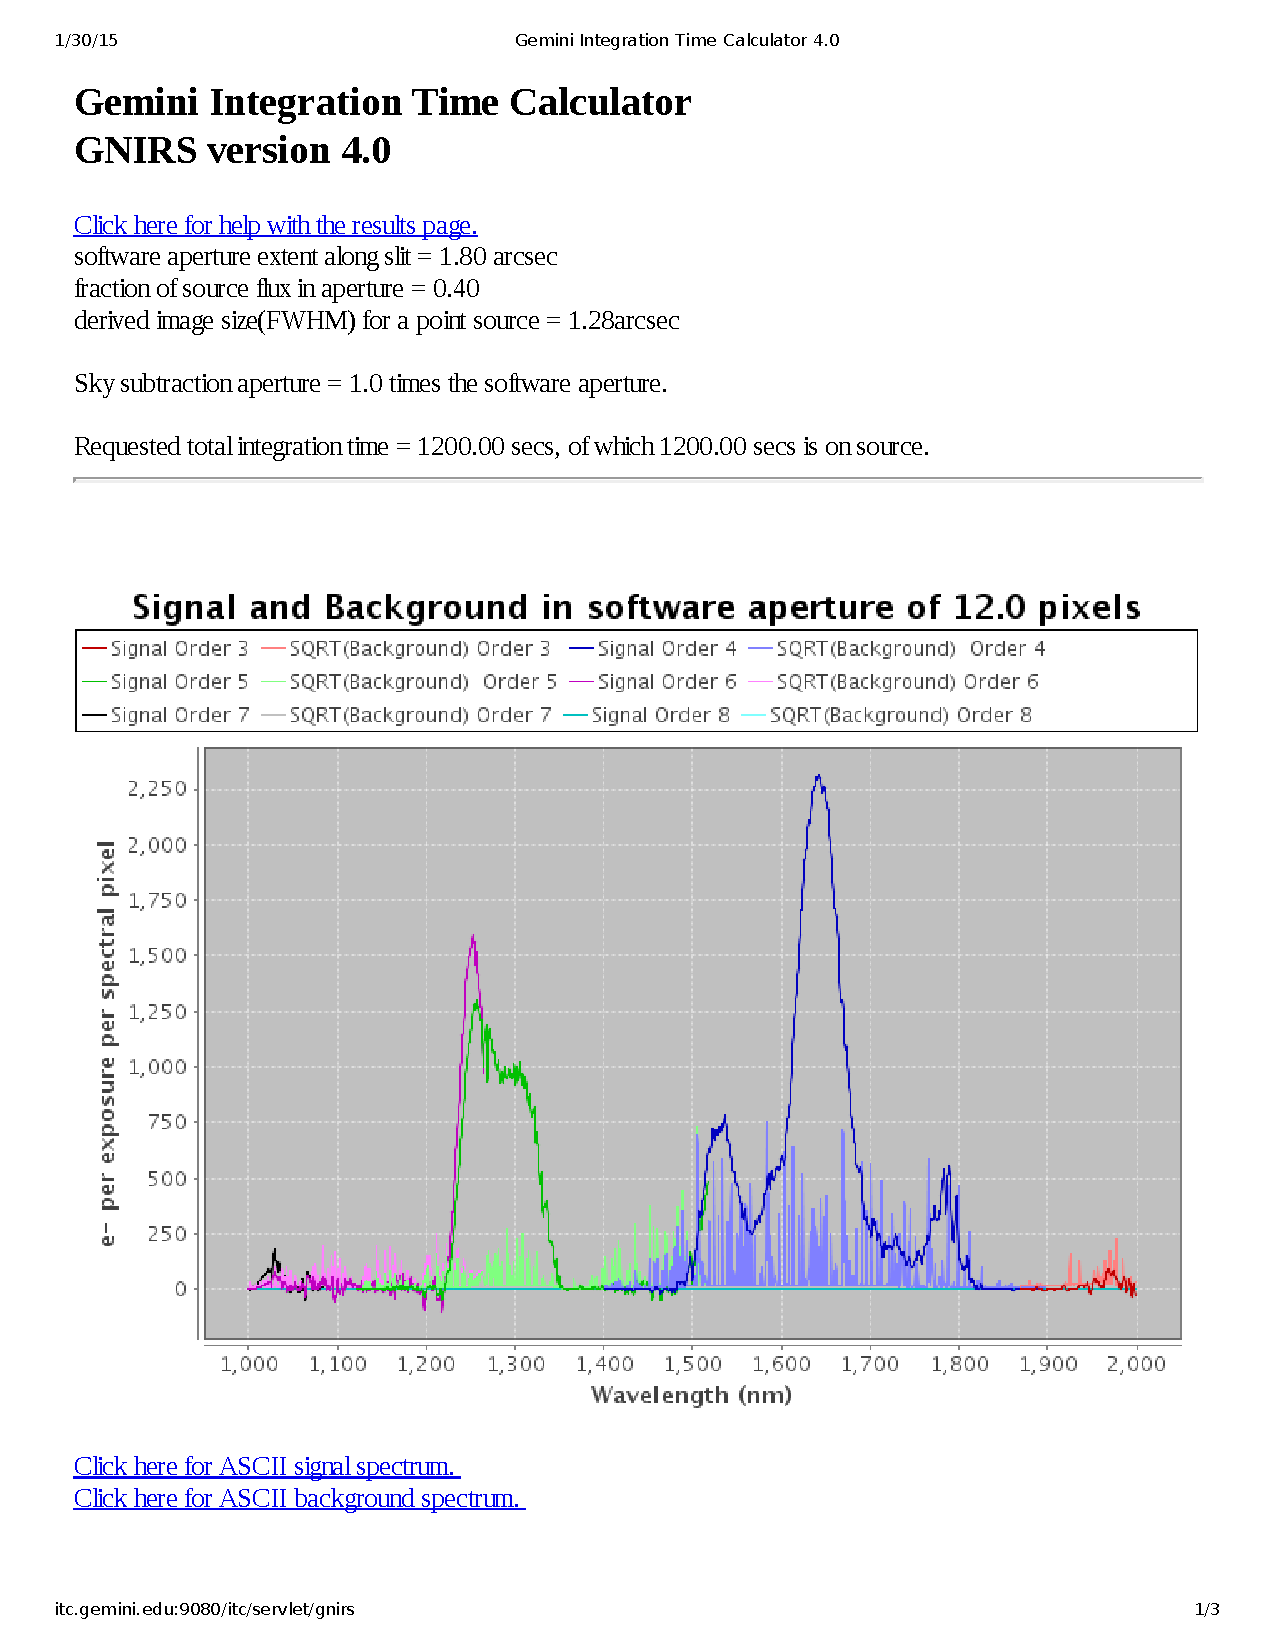
\includepdf[pages={-}]{../itc_14j.pdf}



%%%%%%%%%%%%%%%%%%%%%%%%%%%%%%%%%%%%%%%%%%%%%%%%%%%%%%%%%%%%%%%%%%%%%

% Please do not modify or delete this line.
\end{document}
